\documentclass{classrep}
\usepackage[utf8]{inputenc}

\usepackage[pdftex]{color,graphicx}
\DeclareGraphicsExtensions{.pdf,.png,.jpg,.bmp,.gif}

\usepackage{mathtools}
\usepackage{amsthm}
\usepackage{amsfonts}
\usepackage{float}
\usepackage{subfig}
\usepackage{color}
\usepackage{tabularx}
\usepackage{listings}
\usepackage{indentfirst}
\usepackage{color}
\usepackage{url}
\usepackage{hyperref}
\usepackage[polish]{babel}
\usepackage{paralist}
\usepackage{indentfirst}

\hypersetup{colorlinks=false,pdfborder={0 0 0}}

\definecolor{javared}{rgb}{0.6,0,0} % for strings
\definecolor{javagreen}{rgb}{0.25,0.5,0.35} % comments
\definecolor{javapurple}{rgb}{0.5,0,0.35} % keywords
\definecolor{javadocblue}{rgb}{0.25,0.35,0.75} % javadoc

\lstset{language=Java,
basicstyle=\ttfamily,
keywordstyle=\color{javapurple}\bfseries,
stringstyle=\color{javared},
commentstyle=\color{javagreen},
morecomment=[s][\color{javadocblue}]{/**}{*/},
numbers=left,
numberstyle=\tiny\color{black},
stepnumber=2,
numbersep=10pt,
tabsize=4,
showspaces=false,
showstringspaces=false}

\studycycle{Informatyka, studia dzienne, mgr II st.}
\coursesemester{I}

\coursename{Przetwarzanie obrazu i dźwięku}
\courseyear{2011/2012}

\courseteacher{dr inż. Arkadiusz Tomczyk}
\coursegroup{środa, 8:15}

\author{
  \studentinfo{Paweł Musiał}{178726} \and
  \studentinfo{Łukasz Michalski}{178724}
}
\title{Zadanie 2:\\  \textbf {Filtracja w dziedzinie częstotliwości i segmentacja obrazu.}}
\svnurl{http://serce.ics.p.lodz.pl/svn/labs/poid/at_sr0800/lmpm}

\begin{document}
\maketitle

\addtocounter{footnote}{1}

\tableofcontents

\section{Cel}

Celem zadania było stworzenie aplikacji realizującej poniższe element :
\begin{itemize}
\renewcommand{\labelitemi}{$\bullet$}
\item Zaimplementować proste i odwrotne szybkie przekształcenie Fouriera z decymacją w dziedzinie częstotliwości, a następnie zastosować je do obrazów. Powinna istnieć możliwość obejrzenia zarówno widma mocy, jak i widma fazy.
\item Zaimplementować następujące metody filtracji:
\begin{itemize}
\item (F1) Filtr dolnoprzepustowy (górnozaporowy).
\item (F2) Filtr górnoprzepustowy (dolnozaporowy).
\item (F3) Filtr pasmowoprzepustowy.
\item (F4) Filtr pasmozaporowy.
\item (F5) Filtr z detekcją krawędzi.
\end{itemize}
\item Zaimplementować filtr modyfikujący fazę widma transformaty Fouriera. Modyfikacja ta polega, dla obrazu o wymiarach NxM , na pomnożeniu każdego elementu widma przez:
\begin{equation*}
P(n,m) = \exp \left( j \cdot \left( \frac{-n k 2 \pi}{N} + \frac{-m l 2 \pi }{M} \left( k + l  \right) \pi \right)\right)
\end{equation*}
\item Zaimplementować metodę segmentacji - metoda podziału obszarów \footnote{ang. region splitting and merging}  w celu znalezienia spójnych obszarów o jednolitej barwie. Jako wynik należy wygenerować obrazy reprezentujące znaleziony obszary o jednolitej barwie (tyle masek ile znalezionych obszarów), na których kolorem białym oznaczone są te obszary, a czarnym pozostała część obrazu. Powinna istnieć możliwość nałożenia wybranych masek na obraz przy czym sposób wizualizacji tego nałożenia wybrany powinien zostać przez twórców aplikacji.
\end{itemize}

W sprawozdaniu zamieszczono wyniki działania poszczególnych algorytmów oraz porównanie ich pracy w różnych wariantach ustawień i~dla różnych problemów. Badania przeprowadzono zarówno na obrazach kolorowych (24-bitowych), jak i~w odcieniach szarości (8-bitowych), a~część badań również na obrazach czarno-białych (1-bitowych). 

\section{Wprowadzenie}
Obrazy przechowywane są w pamięci komputera w postaci bitowej, w której określa się ilość bitów przypadającą na każdy piksel obrazu. Kolorowe zdjęcia zapisywane są w formacie 24-bitowym co odpowiada 8-bitom na każdy~z trzech składowych kanałów formatu RGB. Fotografie w odcieniach szarości wykorzystują tylko jeden kanał dlatego wystarczy tutaj przechowywać 8-bitów na każdy zapisany piksel. Taki zapis umożliwia uzyskanie 256 różnych wartość danego piksela czyli 256 różnych odcieni szarości poczynając od białego na kolorze czarnym kończąc. W przypadku obrazów kolorowych liczba kombinacji jest dużo większa i wynosi 16,777,216, co nie oznacza, że wszystkie uzyskane w ten sposób kolory są między sobą rozróżnialne. W tej pracy wszystkie przygotowane algorytmy operują na poszczególnych wartościach każdego kanału obrazu.

\subsection{Filtracja w dziedzinie częstotliwości}

Filtracja w dziedzinie częstotliwości analogicznie jak w przypadku analizowanego w poprzednim zadaniu, polega na przemnożeniu danych przez jakiś filtr $H(k)$.  W większości przypadków udało się uzyskać filtrację idealną jak i filtrację z przejściem ciągłym. Co w pewnych przypadkach dawało bardziej zadowalające efekty.\\ Opisując metody filtracji będziemy posługiwać się poniższymi oznaczeniami :
\begin{itemize}
\item $D(u,v)$ odległość częstotliwości $(u,v)$ od częstotliwości maksymalnej
\item $D_0$ częstotliwość progowa
\item $D_L$ $D_H$ - dolna, górna częstotliwość progowa
\item $n$ - parametr filtru Butterwortha.
\end{itemize}

Działanie filtrów demonstrowane będzie na przykładzie obrazu \emph{lena.bmp} \footnote{\url{http://ics.p.lodz.pl/~tomczyk/available/po/images/lena.bmp}}.

\subsubsection{Algorytm szybkiej transformaty Fouriera}

Postać ogólna dyskretnej transformaty Fouriera \ref{DFT} oraz jej odwrotność \ref{IDFT}
\begin{eqnarray}
\label{DFT}  X(k) = \sum \limits ^{N-1} _{n=0} x(n) W ^{kn} _{N}\\
\label{IDFT}  x(k) = \frac{1}{N} \sum \limits ^{N-1} _{n=0} X(n) W ^{-kn} _{N}
\end{eqnarray}
gdzie $W _N  = e^{j2 \pi / N}$ .

Złożoność obliczeniowa tego przekształcenia w postaci powyżej przedstawionej jest wyższa od liniowej a zasadniczo kwadratowej ($N^2$), co nie jest zadowalającym wynikiem, gdybyśmy chcieli zastosować to przekształcenie na bardzo dużej ilości próbek zdyskretyzowanego sygnału. Jednakże dzięki właściwościom tego przekształcenia możliwa jest jego optymalizacja.

Poniżej przedstawiony algorytm szybkiej transformaty Fouriera(\emph{FFT)} z decymacją w częstotliwości. W algorytmie tym rozdzielamy przekształcenie na dwa podrzędne operujące na połówkach danych podstawowych uzyskując \ref{FFT_1}. Następnie rozdzielamy operacje dla parzystych i nie parzystych próbek, uzyskując postacie \ref{FFT_1even}, \ref{FFT_2odd}. 

\begin{multline}
X(k) = \sum \limits ^{N/2-1} _{n=0} x(n) W ^{kn} _{N} + \sum \limits ^{N/2-1} _{n=0} x(n) W ^{kn} _{N} = \\
= \sum \limits ^{N/2-1} _{n=0} x(n) W ^{kn} _{N} + W ^{N k/2} _{N} \sum \limits ^{N/2-1} _{n=0} x \left( n + \frac{N}{2} \right) W ^{kn} _{N} \\
\label{FFT_1} X(k) = \sum \limits ^{N/2-1} _{n=0} \left[ x(n) + (-1) ^{k} x(n+\frac{N}{2} ) \right]W ^{kn} _{N}
\end{multline}

\begin{eqnarray}
\label{FFT_1even} X(2k) = \sum \limits ^{N/2-1} _{n=0} \left[ x(n) + x \left(  n+\frac{N}{2} \right)  \right]\\
\label{FFT_2odd} X(2k+1) = \sum \limits ^{N/2-1} _{n=0} \left\{ \left[ x(n) - x \left(  n+\frac{N}{2} \right) \right] \right\}
\end{eqnarray}
gdzie użyto faku, iż $W _N ^2  = W _{N/2}$.

Algorytm ten opiera się na metodzie programowania ,,dziel i zwyciężaj'' w której dzielimy zbiór danych w kolejnych krokach, uzyskując pod problemy łatwiejsze do rozwiązania a sumarycznie dające wynik przekształcenia na zbiorze sprzed podziału. Po zastosowaniu wyżej opisanej optymalizacji przekształcenia podstawowego \ref{DFT}, algorytm swoją złożoność $N \log _{2} N$.Dokładniejszy opis algorytmu można znaleźć w \cite{1}.

Powyżej opisano jedynie algorytm prostego przekształcenia Fouriera, ponieważ algorytm dla przekształcenia odwrotnego będzie wyglądał analogicznie do opisanego tutaj, zmiany dotyczyć będą widocznych na pierwszy rzut oka różnic pomiędzy \ref{DFT} i \ref{IDFT}.

W naszym przypadku jednak mamy do czynienia z obrazem dwuwymiarowym, nie wektorem jednowymiarowym. Jednak dzięki własnościom transformaty Fouriera, możemy po prostu obliczyć transformate wektorów wierszowych a następnie kolumnowych, aby uzyskać pożądany wynik. Przekształcenie to transformuje dyskretne dane z przestrzeni $\mathcal{R} \rightarrow \mathcal{C}$, ważniejszym jednak będzie dla nas co przekształcone dane sobą prezentują, czyli przestrzeń częstotliwości danego sygnału wejściowego.

\begin{figure}[H]
  \centering
  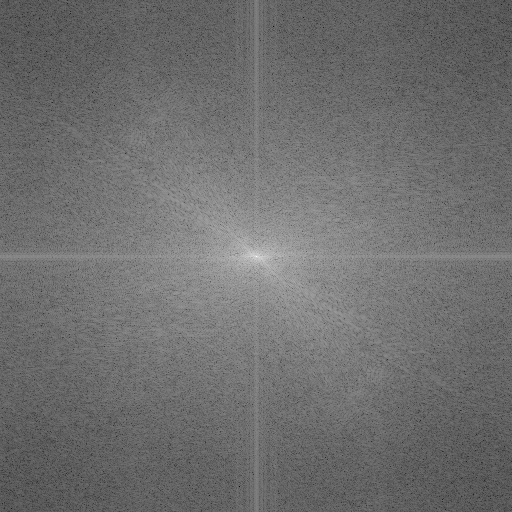
\includegraphics[width=0.5\textwidth]{img/lena_orig}
  \caption{Widmo mocy obrazu \emph{lena.bmp}.}
  \label{fig_widmo_lena_orig}
\end{figure}


\subsubsection{Filtr dolnoprzepustowy}

Filtr idealny.
\begin{equation}
  H_{lp} (u,v) = \left\{
  \begin{array}{l l}
    1 & \quad dla\ D(u,v) \leq D_0 \\
    0 & \quad dla\ D(u,v) > D_0 \\
  \end{array} \right.
\end{equation}

Filtr ciągły - Butterwortha \footnote{Butterworth}.
\begin{equation}
H_{lp}(u,v) = \frac{1}{1+ \left[ D(u,v) / D_0\right] ^{2n} }
\end{equation}

 \begin{figure}[H]
  \centering
  \subfloat[filtr idealny]{
	  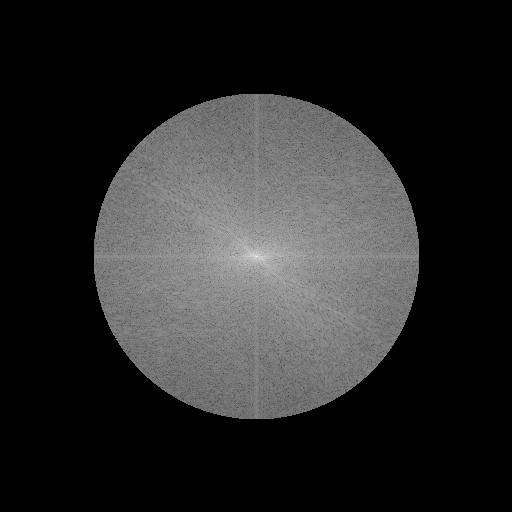
\includegraphics[width=0.4\textwidth]{img/lena_lowpass}
  }
  \subfloat[filtr Butterwortha]{
  		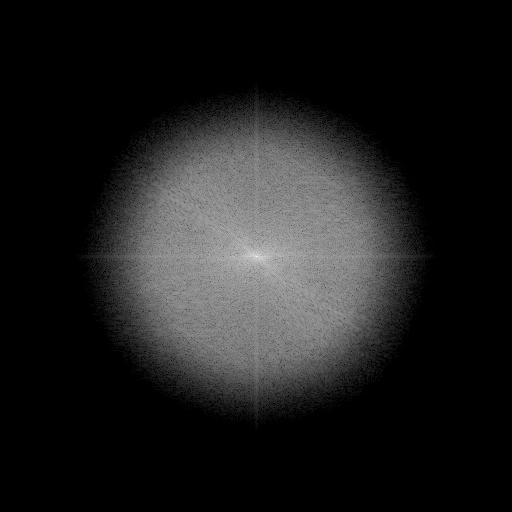
\includegraphics[width=0.4\textwidth]{img/lena_lowpassB}
  	}
  \caption{Filtr dolnoprzepustowy, widmo mocy.}
  \label{fig_widmo_lena_lp}
\end{figure}

\subsubsection{Filtr górnoprzepustowy}

Filtr idealny.
\begin{equation}
  H_{hp}(u,v) = \left\{
  \begin{array}{l l}
    1 & \quad dla\ D(u,v) \geq D_0 \\
    0 & \quad dla\ D(u,v) < D_0 \\
  \end{array} \right.
\end{equation}

Filtr ciągły - Butterwortha.
\begin{equation}
H_{hp}(u,v) = 1 - H_{lp}(u,v)
\end{equation}

 \begin{figure}[H]
  \centering
  \subfloat[filtr idealny]{
	  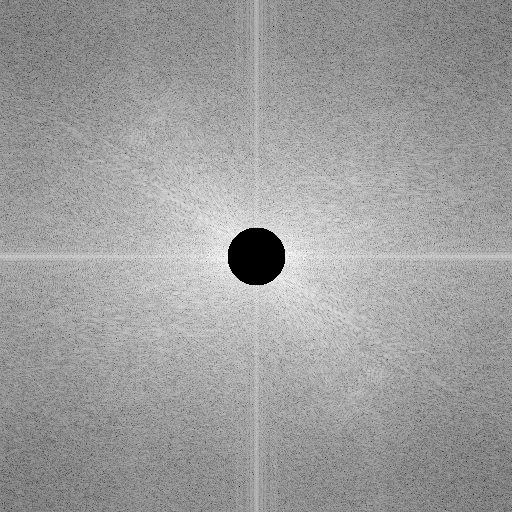
\includegraphics[width=0.4\textwidth]{img/lena_highpass}
  }
  \subfloat[filtr Butterwortha]{
  		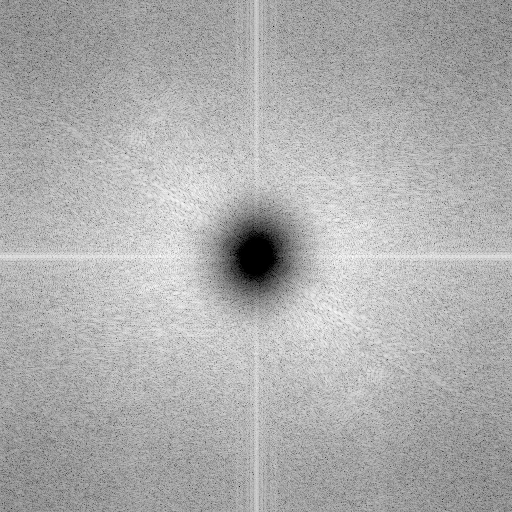
\includegraphics[width=0.4\textwidth]{img/lena_highpassB}
  	}
  \caption{Filtr dolnoprzepustowy, widmo mocy.}
  \label{fig_widmo_lena_hp}
\end{figure}

\subsubsection{Filtr pasmowoprzepustowy}

Filtr idealny.
\begin{equation}
  H_{hp}(u,v) = \left\{
  \begin{array}{l l}
    1 & \quad dla\ D_L \leq D(u,v) \leq D_H \\
    0 & \quad inny\ przypadek \\
  \end{array} \right.
\end{equation}

Filtr ciągły - Butterwortha.
\begin{eqnarray}
H_{lp}(u,v) = \frac{1}{1+ \left[ D(u,v) / D_L\right] ^{2n} }\\
H_{hp}(u,v) =1 - \frac{1}{1+ \left[ D(u,v) / D_H\right] ^{2n} }\\
H_{bp}(u,v) = H_{lp}(u,v) \cdot H_{hp}(u,v)
\end{eqnarray}

 \begin{figure}[H]
  \centering
  \subfloat[filtr idealny]{
	  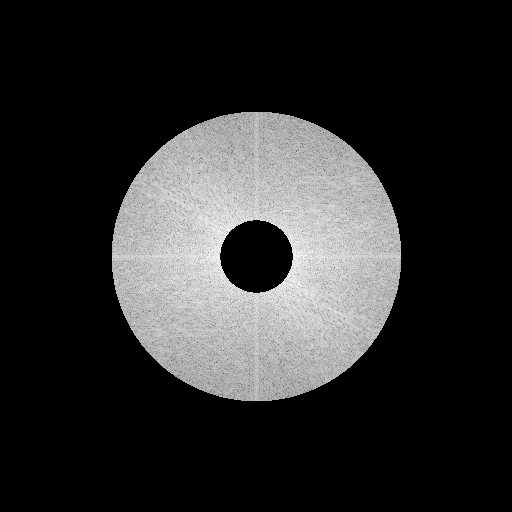
\includegraphics[width=0.4\textwidth]{img/lena_bandpass}
  }
  \subfloat[filtr Butterwortha]{
  		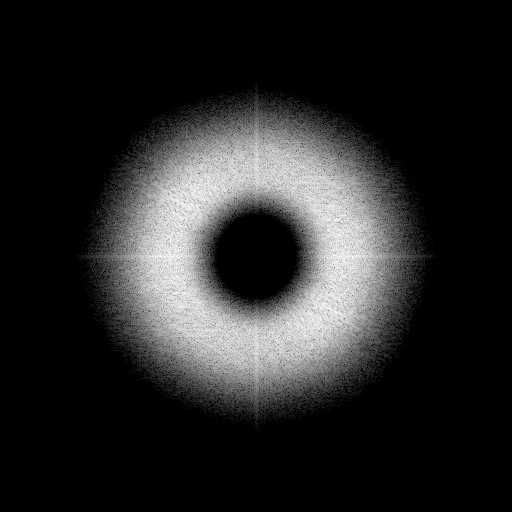
\includegraphics[width=0.4\textwidth]{img/lena_bandpassB}
  	}
  \caption{Filtr dolnoprzepustowy, widmo mocy.}
  \label{fig_widmo_lena_bp}
\end{figure}

\subsubsection{Filtr pasmowozaporowy}

Filtr idealny.
\begin{equation}
  H_{bs}(u,v) = \left\{
  \begin{array}{l l}
    0 & \quad dla\ D_L \leq D(u,v) \leq D_H \\
    1 & \quad inny\ przypadek \\
  \end{array} \right.
\end{equation}

Filtr ciągły - Butterwortha.
\begin{equation}
H_{bs}(u,v) = 1 - H_{bp}(u,v)
\end{equation}

 \begin{figure}[H]
  \centering
  \subfloat[filtr idealny]{
	  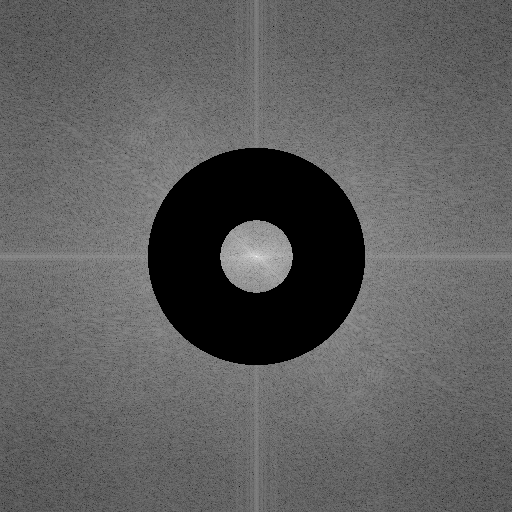
\includegraphics[width=0.4\textwidth]{img/lena_bandstop}
  }
  \subfloat[filtr Butterwortha]{
  		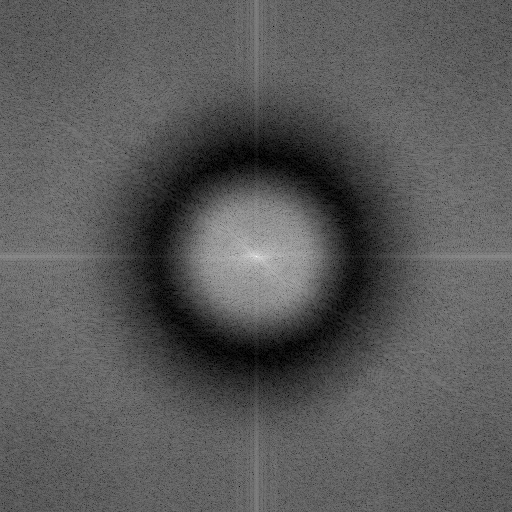
\includegraphics[width=0.4\textwidth]{img/lena_bandstopB}
  	}
  \caption{Filtr dolnoprzepustowy, widmo mocy.}
  \label{fig_widmo_lena_bs}
\end{figure}

\subsubsection{Filtr z detekcją krawędzi}

Filtracja ta jest jakby modyfikacją filtru pasmowoprzepustowego. Ponieważ z pasma wydzielonego przez filtr $H_{bp}$ wycinamy symetrycznie względem maksymalnej częstotliwości łuki o pewnym kącie $\alpha$. Dla jasności najlepiej zobrazować widmo mocy sygnału.

\begin{figure}[H]
  \centering
  
\includegraphics[width=0.5\textwidth]{img/lena_edge_detect}
  \caption{Filtr z detekcją krawędzi, widmo mocy.}
  \label{fig_widmo_lena_edge_detect}
\end{figure}


\subsubsection{Filtr modyfikujący widmo}

\begin{equation}
\label{eq:modyfikacja}
H(u,v) = \exp { \left( j \cdot \left( \frac{-u k 2 \pi}{N} + \frac{-v l 2 \pi }{M} \left( k + l  \right) \pi \right)\right) }
\end{equation}

\begin{figure}[H]
  \centering
  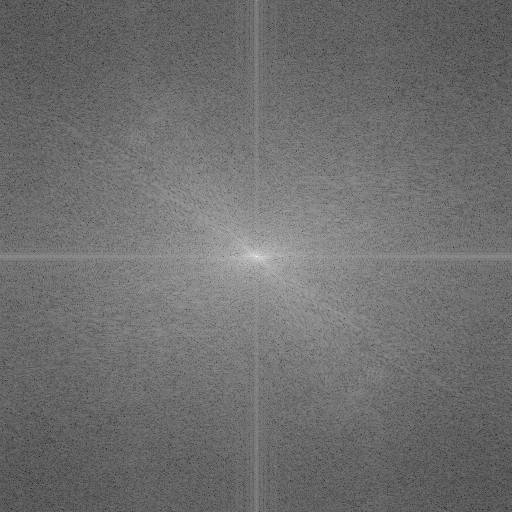
\includegraphics[width=0.5\textwidth]{img/lena_spectreMod}
  \caption{Filtr modyfikujący widmo, widmo mocy.}
  \label{fig_widmo_lena_spectreMod}
\end{figure}


\subsection{Segmentacja}
Nasza grupa miała zadanie zrealizować segmentacje opartą o podział obrazu na rejony a następnie ich łączenie. Wykorzystaliśmy w tym celu drzewa czwórkowe do przechowywania danych. Sam algorytm segmentacji jest dość prosty i składa się z kilku kroków:
\begin{enumerate}
\item Należy sprawdzić czy podany obszar obrazu jest jednolity przy pomocy wcześniej zdefiniowanej funkcji porównującej wartości poszczególnych piksli.
\item Jeśli warunek z punktu pierwszego nie zachodzi należy ten obszar podzielić na cztery równe części i powtórzyć całą operację dla każdej z nich.
\item Jeżeli podany obszar jest jednolity jest on dodawany do listy i jego przetwarzanie jest zakończone.
\item Dla tak uzyskanych obszarów wyliczany jest średni kolor, który reprezentuje każdy z nich.
\item Na podstawie średniego koloru następuje łączenie obszarów, które są podobne do siebie wykorzystując funkcję sprawdzającą spójność z punktu 1.
\end{enumerate}

W punkcie pierwszym algorytmu wykorzystuje się do testowania spójności obszarów dowolnie zdefiniowaną funkcję porównującą wartości dwóch podanych pikseli. Dzięki dodaniu pewnej tolerancji tej różnicy można uzyskać obszary o podobnej charakterystyce. Sam algorytm rozpoczyna swoje działanie sprawdzając czy cały obszar obrazu jest spójny i kontynuując swoją pracę dzieli go na mniejsze części.

Po uzyskaniu już wszystkich jednolitych obszarów następuje ich łączenie w większe rejony zawierające w sobie obszary o podobnej charakterystyce. Dzięki temu zmniejsza się ilość poszczególnych pojedynczych komórek. Ten etap jest ważny z punktu widzenia tego algorytmu segmentacji. Jednak problem optymalnego znajdowania sąsiadów w drzewach czwórkowych nie jest trywialny. W tym celu wykorzystaliśmy algorytm QTLCLD \cite{3} umożliwiający poprzez specjalną architekturę poszczególnych węzłów tego drzewa na znajdowanie sąsiadów w stałym czasie.

Algorytm QTLCLD opisany w \cite{3} stanowi podobne podejście jak czwórkowe drzewa liniowe, dzięki czemu czas znajdowania sąsiadów poszczególnych liści takiego drzewa jest znacznie krótszy niż w przypadku algorytmów przeglądając całą jego strukturę. 

Główną zastosowaną tutaj zasadą jest przypisywanie odpowiednim komórką takiego drzewa specjalnych kodów dzięki, którym można określić ich pozycję w całej strukturze. Zostało to przedstawione na rysunku \ref{fig_seg_kody}.

\begin{figure}[H]
  \centering
  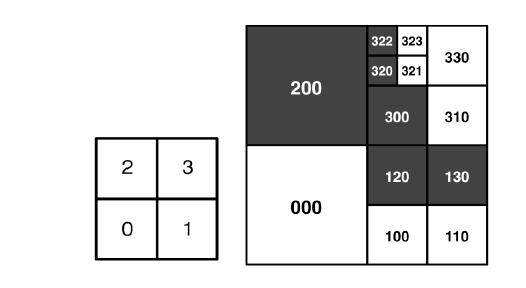
\includegraphics[width=0.8\textwidth]{img/seg/kody}
  \caption{Kody poszczególnych obszarów dla maksymalnego zagłębienia wynoszącego 3. Źródło \cite{3}.}
  \label{fig_seg_kody}
\end{figure}

Schemat przypisywania poszczególnych numerów z zakresu [0,3] został przedstawiony na pierwszej części rysunku \ref{fig_seg_kody} i jest on ustalany w trakcie podziału obszaru rodzica. Każde z dzieci dziedziczy po swoim rodzicu jego kod dodając na kolejnej pozycji określonej przez głębokość w drzewie na jakiej się znajduje swój własny indeks. Dzięki takiemu systemowi można łatwo zlokalizować położenie danego obszaru w całym drzewie oraz określić na jakiej głębokości się on znajduje. 

Jednak by umożliwić sprawne i szybkie odnajdowanie sąsiadów danego obszaru należało dodać kolejny zestaw wartości tym razem określający różnice wielkości między danym obszarem a czterema jego sąsiadami. Wartości te są wyliczane w trakcie budowania drzewa, który to proces oparty jest o algorytm BFS. Na rysunku \ref{fig_seg_kody2} przedstawiono przykładowe powstałe w ten sposób drzewo reprezentujące cały obraz. Jego maksymalne zagłębienie wynosi w tym przypadku 3.

\begin{figure}[H]
  \centering
  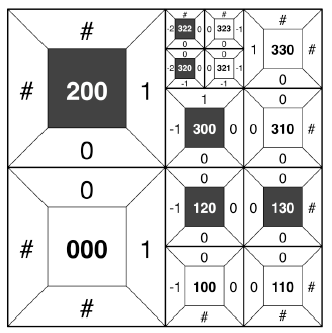
\includegraphics[width=0.5\textwidth]{img/seg/kody2}
  \caption{Kody poszczególnych obszarów wraz z różnicą wielkości do sąsiadów. Źródło \cite{3}.}
  \label{fig_seg_kody2}
\end{figure}

Wykorzystując tak przygotowaną strukturę łatwo można uzyskać kod sąsiada danego obszaru w danym kierunku przy pomocy wzoru:
\begin{equation}
\label{eq:seg_nei}
m_{q}=\left\{
\begin{array}{lcc}
((n_{q}>>2(r-l-dd))<<2(r-l-dd))\oplus_{q}(\Delta n_{d}<<(2(r-l-dd)))&\mbox{dla}&dd<0\\
n_{q}\oplus_{q}(\Delta n_{d}<<(2(r-l)))&\mbox{dla}&dd\ge 0
\end{array}
\right.
\end{equation}
gdzie:
\begin{itemize}
\item $m_{q}$ - poszukiwany kod obszaru sąsiedniego
\item $n_{q}$ - kod obszaru bazowego
\item $r$ - maksymalna głębokość drzewa
\item $dd$ - różnica wielkości między obszarem bazowym a sąsiadem w zadanym kierunku
\item $l$ - poziom zagłębienia na jakim znajduje się bazowy obszar
\item $d$ - kierunek poszukiwań sąsiada z przedziału $[0,3]$
\item $n_{d}$ - stała wartość dla odpowiedniego kierunku $d$ i maksymalnego poziomu drzewa
\end{itemize}

Algorytm ten opiera się w dużej mierze na algorytmie Scharcka skąd wywodzi się użyty operator $\oplus_{q}$ zdefiniowany jak poniżej:
\begin{equation}
n_{q}\oplus_{q}k_{q} = (((n_{q}|t_{y})+(k_{q}\wedge t_{x}))\wedge t_{x})|(((n_{q}|t_{x})+(k_{q}\wedge t_{y}))\wedge t{y})
\end{equation}
gdzie:
\begin{itemize}
\item $|$ - oznacza operację bitową OR
\item $\wedge$ - oznacza operację bitową AND
\item $+$ - jest normalny dodawaniem dwóch liczby
\end{itemize}

Dodatkowo we wzorze pojawiają się dwie stałe $t_{x}$ i $t_{y}$,które są zdefiniowane następująco:
\begin{equation*}
\begin{array}{cc}
t_{x} = 01..0101& \mbox{,,01'' powtórzone $r$ razy}\\
t_{y} = 10..1010& \mbox{,,10'' powtórzone $r$ razy}
\end{array}
\end{equation*}
gdzie:
\begin{itemize}
\item $r$ - maksymalna głębokość drzewa
\end{itemize}

Stałe $n_{d}$ dla czterech kierunków poszukiwań użyte w równaniu \ref{eq:seg_nei} określone są następująco:
\begin{equation*}
\begin{array}{lc}
n_{1} = 00..01& \mbox{wschodni sąsiad}\\
n_{1} = 00..10& \mbox{północy sąsiad}\\
n_{2} = t_{y}& \mbox{zachodni sąsiad}\\
n_{3} = t_{x}& \mbox{południowy sąsiad}\\
\end{array}
\end{equation*}
Stałe $n_{1}$ i $n_{1}$ są uzupełniane zerami tak aby łączna ich długość bitów wynosiła $2r$.

Analizując równanie \ref{eq:seg_nei} łatwo można dojść do wniosku, że czas potrzebny na wyznaczenie sąsiada danego obszaru jest słały bez względu na wielkość i złożoność drzewa. Za każdym bowiem razem ilość operacji jakie należy wykonać jest taka sama. 

Jedynym ograniczeniem przyjętego rozwiązania jest fakt, że znajduje ono sąsiadów o takim samym rozmiarze co obszar bazowy lub większych. Nie stanowi to jednak problemu w naszym zadaniu gdyż nawet ta informacja pozwala z powodzeniem na sprawdzenie wszystkich obszarów wygenerowanego drzewa.
\section{Opis implementacji}
W samej implementacji aplikacji nie zaszły znaczące zmiany w porównaniu do zadania pierwszego. Wykorzystaliśmy ten sam szkielet dodając nowe funkcję i opcję w menu. 

Implementacja filtracji i wszystkich rodzajów filtrów została przeprowadzona poprzez wcześniej dostępny interfejs \textit{IFilter} i nie różni się znacząco od tej opisanej w zadaniu pierwszym. Dodana została przez to nowa opcja w głównym menu programu umożliwiająca zaaplikowanie wybranego rodzaju filtracji do zadanego obrazu. Dodatkowo zostało przygotowane osobne okno służące do wyświetlenia obrazów widma mocy uzyskanych poprzez FFT. Stanowi ono pomoc przy doborze parametrów filtrów oraz obrazuje ich pracę.

Poszczególne metody i funkcję wykorzystane przy procesie filtracji zostały umieszczone w klasie pomocniczej \textit{FFTTools}. Umożliwia to ich ponowne wykorzystanie w innym projekcie oraz stosunkowo prostą rozbudowę lub wprowadzenie zmian.

W przypadku drugiej części zadania dotyczącej segmentacji obrazu uznaliśmy, że wcześniej przygotowane narzędzia nie umożliwią jej poprawnej realizacji. Dlatego zostało dodane nowe okno dostępne w menu \textit{Other} w głównym oknie programu. 
\begin{figure}[H]
  \centering
  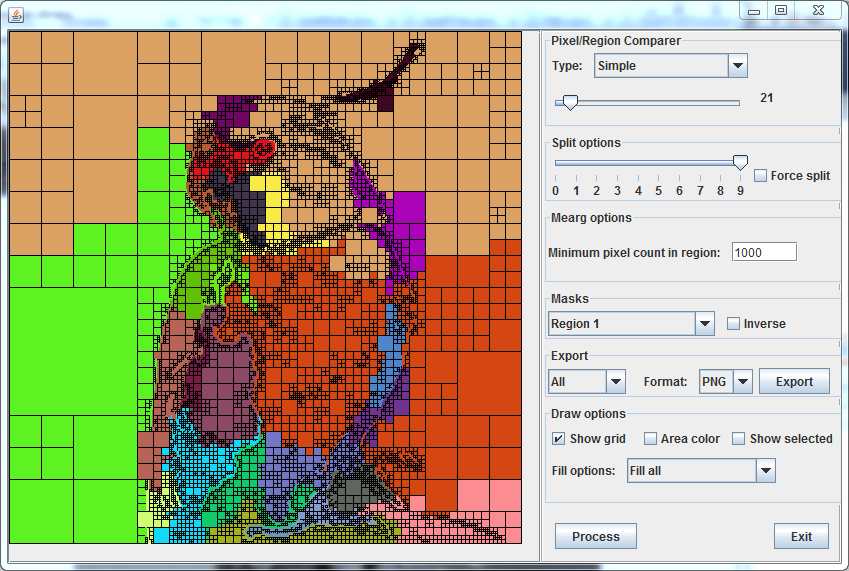
\includegraphics[width=\textwidth]{img/seg/segWindow}
  \caption{Okno segmentacji obrazu.}
  \label{fig_seg_window}
\end{figure}

Okno to zawiera z prawej strony szereg opcji, dzięki którym możemy określić parametry procesu segmentacji jak i już wizualizacji osiągniętych wyników. Możemy wybrać różne metody porównywania pikseli oraz ustawić tolerancję różnicy wartości między nimi. Obecnie dostępne są trzy wariant: 
\begin{enumerate}
\item Metryka Euklidesowa
\begin{equation*}
D = \sqrt{(R_{1}-R_{2})^2+(G_{1}-G_{2})^2+(B_{1}-B_{2})^2}
\end{equation*}
\item Porównanie jasności
\begin{equation*}
\begin{array}{l}
y = 0,299R + 0,587G + 0,114B\\
D = |y_{1}-y_{2}|
\end{array}
\end{equation*}
\item Porównanie osobno każdego kanału
\begin{equation*}
D =\max\left(|R_{1}-R_{2}|, |G_{1}-G_{2}|, |B_{1}-B_{2}|\right)
\end{equation*}
\end{enumerate}
gdzie indeks przy literze określa numer porównywanego piksela a litery $R, G, B$ odpowiednim kanałom jego koloru. Oczywiście dla obrazów w skali szarości wszystkie te wzory redukują się do porównywania jedynie jednego kanału.

Można również ustawić maksymalną głębokość drzewa. Wtedy podział następuje nie głębiej niż podany limit. Jeśli chcę się uzyskać równą siatkę z obszarami o takim samym poziomie zagłębienia można zaznaczyć opcję \textit{force}. Kolejny etap algorytmu realizuje łączenie obszarów w rejony. W naszej aplikacji istnieje możliwość określenia w pikselach minimalnej wielkość tak uzyskanego rejonu. Dzięki temu można ograniczyć ilość powstałych masek.

Okno segmentacji wspiera również różne metody podglądu osiągniętego rezultatu oraz możliwość eksportu powstałych masek do plików graficznych w formacie binarnym. 

\section{Wyniki}

\subsection{Filtracja w dziedzinie częstotliwości}

Widma mocy jak i również fazy, nie będą prezentowane przy okazji prezentowania wyników filtracji, zostały one przedstawione przy okazji wyjaśnienia działania poszczególnych filtrów. Powodem tego jest fakt, iż widma obrazów naturalnych są trudne do interpretacji, natomiast dla obrazów sztucznych, np wzorców są one znacznie bardziej przejrzyste dla naszego oka.

Dla przykładu, widmo przypadkowego obrazu prezentującego pewien wzorzec \ref{fig_pattern}, i obrazu naturalnego \ref{fig_widmo_lena_orig}.

 \begin{figure}[H]
  \centering
  \subfloat[obraz]{
	  
\includegraphics[width=0.4\textwidth]{img/pattern}
  }
  \subfloat[widmo mocy]{
  		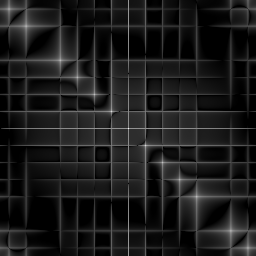
\includegraphics[width=0.4\textwidth]{img/pattern_widmo}
  	}
  \caption{Widmo mocy obrazu sztucznego.}
  \label{fig_pattern}
\end{figure}




\subsubsection{Filtr dolnoprzepustowy}



 \begin{figure}[H]
  \centering
  \subfloat[filtr idealny]{
    \label{fig_wyniki:lpA}
	  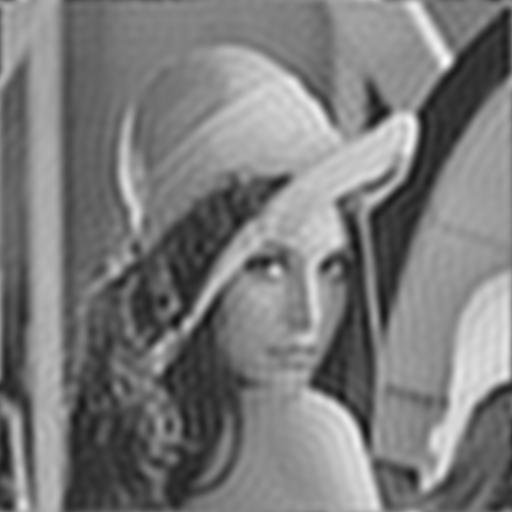
\includegraphics[width=0.42\textwidth]{img/lowpass/lena_N_D0=01}
  }
  \subfloat[filtr Butterwortha n=5]{
    \label{fig_wyniki:lpB}
  		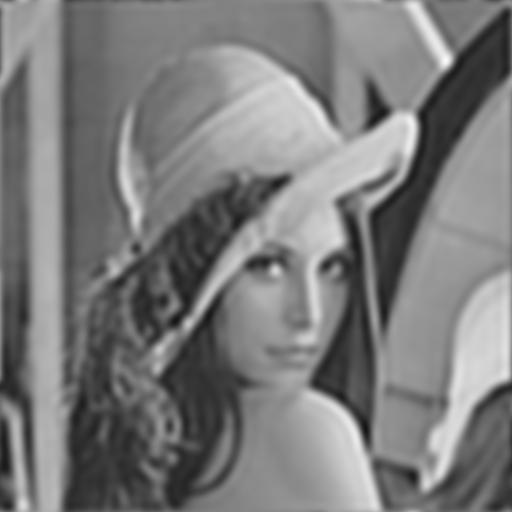
\includegraphics[width=0.42\textwidth]{img/lowpass/lena_D0=01_K=5}
  	}
  \caption{Filtr dolnoprzepustowy, próg $D_0=0.1$.}
  \label{fig_wyniki:lp}
\end{figure}




\subsubsection{Filtr górnoprzepustowy}



 \begin{figure}[H]
  \centering
  \subfloat[$D_0=0.1$]{
    \label{fig_wyniki:hpA}
	  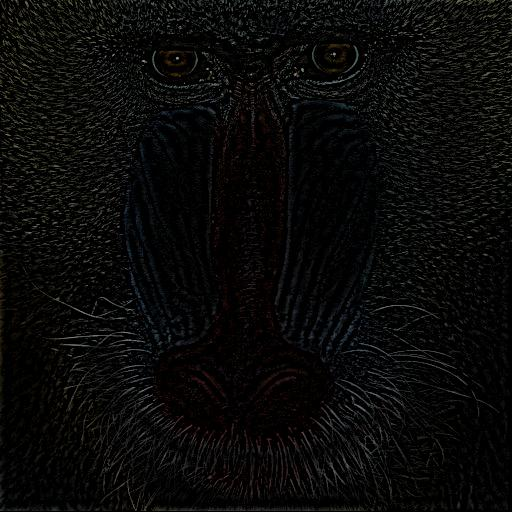
\includegraphics[width=0.42\textwidth]{img/highpass/mandrilc_D0=01}
  }
  \subfloat[$D_0=0.02$, jasność +80]{
    \label{fig_wyniki:hpB}
  		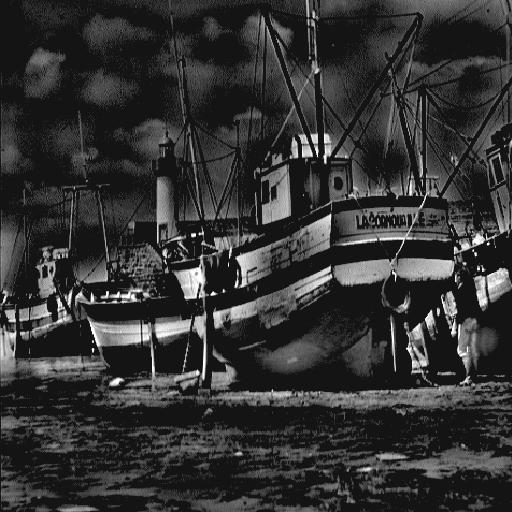
\includegraphics[width=0.42\textwidth]{img/highpass/boat_D0=002_brightness=80}
  	}
  \caption{Filtr górnoprzepustowy.}
  \label{fig_wyniki:hp}
\end{figure}




\subsubsection{Filtr pasmowoprzepustowy}




 \begin{figure}[H]
  \centering
  \subfloat[$D_L=0.03$, $D_H=0.6$, +100 jasność, filtr idealny]{
    \label{fig_wyniki:bp_boatA}
	  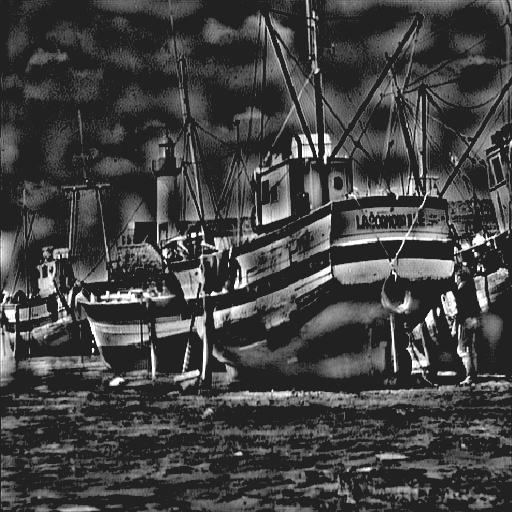
\includegraphics[width=0.42\textwidth]{img/bandpass/boat_DL=003_DH=06_brightness=100}
  }
  \subfloat[$D_L=0.03$, $D_H=0.6$, +100 jasność, filtr Butterwortha n=5]{
    \label{fig_wyniki:bp_boatB}
  		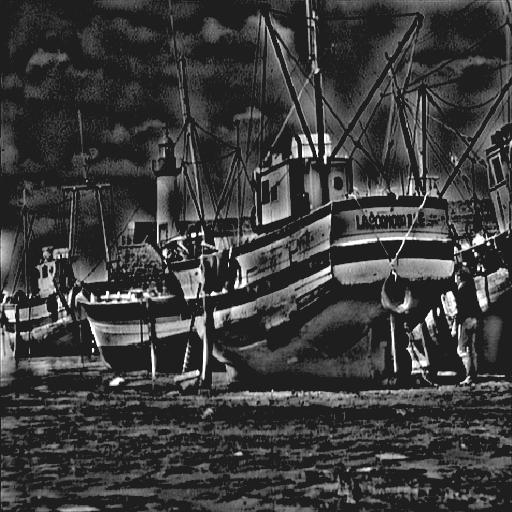
\includegraphics[width=0.42\textwidth]{img/bandpass/boat_DL=003_DH=06_K=5_brightness=100}
  	}
  \caption{Filtr pasmowoprzepustowy.}
  \label{fig_wyniki:bp_boat}
\end{figure}




 \begin{figure}[H]
  \centering
  \subfloat[$D_L=0.01$, $D_H=0.6$, +80 jasność, filtr idealny]{
    \label{fig_wyniki:bp_lenaA}
	  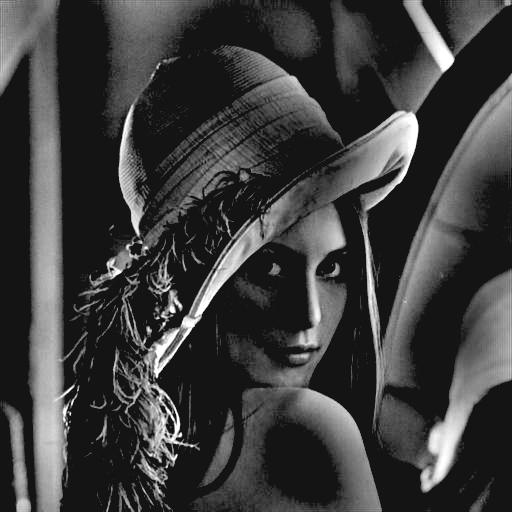
\includegraphics[width=0.42\textwidth]{img/bandpass/lena_DL=001_DH=06_brightness=80}
  }
  \subfloat[$D_L=0.01$, $D_H=0.6$, +80 jasność, filtr Butterwortha n=2]{
    \label{fig_wyniki:bp_lenaB}
  		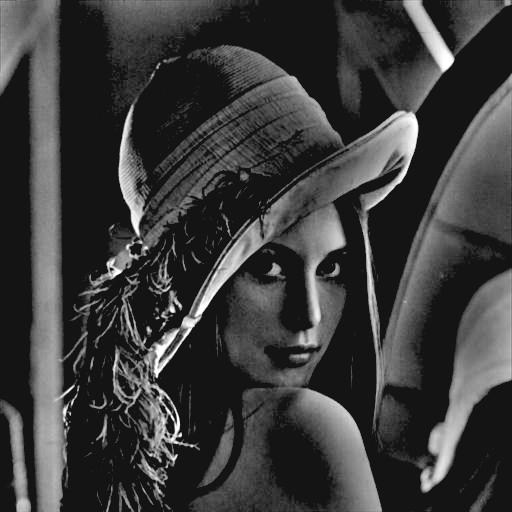
\includegraphics[width=0.42\textwidth]{img/bandpass/lena_DL=001_DH=06_K=2_brightness=80}
  	}
  \caption{Filtr pasmowoprzepustowy.}
  \label{fig_wyniki:bp_lena}
\end{figure}




\subsubsection{Filtr pasmowozaporowy}




 \begin{figure}[H]
  \centering
  \subfloat[$D_L=0.02$, $D_H=0.05$,  filtr idealny]{
    \label{fig_wyniki:bsA}
	  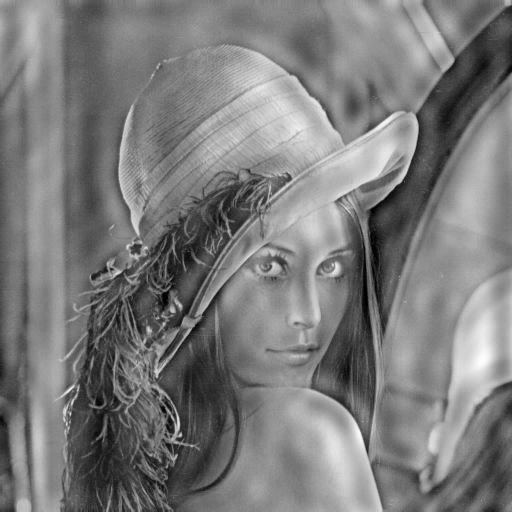
\includegraphics[width=0.42\textwidth]{img/bandstop/lena_DL=002_DH=005}
  }
  \subfloat[$D_L=0.02$, $D_H=0.05$, filtr Butterwortha n=2]{
    \label{fig_wyniki:bsB}
  		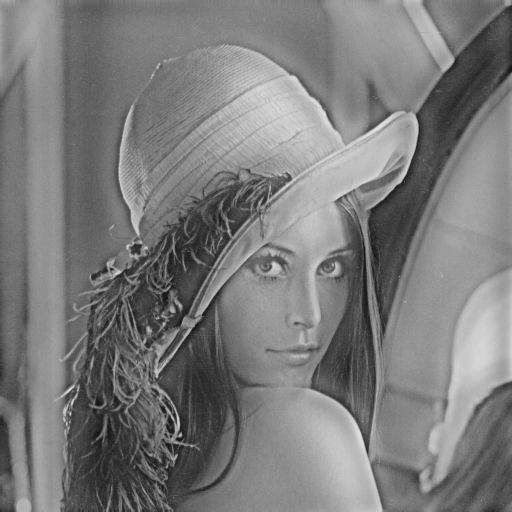
\includegraphics[width=0.42\textwidth]{img/bandstop/lena_DL=002_DH=005_K=2}
  	}
  \caption{Filtr pasmowozaporowy.}
  \label{fig_wyniki:bs}
\end{figure}



\subsubsection{Filtr z detekcją krawędzi}



 \begin{figure}[H]
  \centering
  \subfloat[$D_L=0.15$, $D_H=0.6$, $\alpha = 90 \deg$, $P(0;1)$]{
    \label{fig_wyniki:edgeA}
	  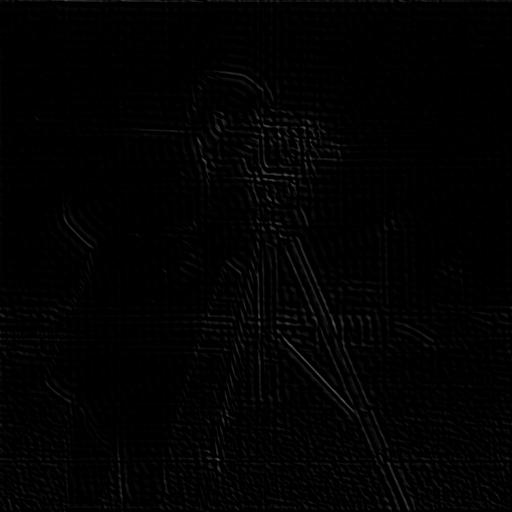
\includegraphics[width=0.32\textwidth]{img/edge_detect/camera_DL=015_DH=06_A=90_P=01}
  }
  \subfloat[$D_L=0.15$, $D_H=0.6$, $\alpha = 90 \deg$, $P(1;0)$]{
    \label{fig_wyniki:edgeB}
  		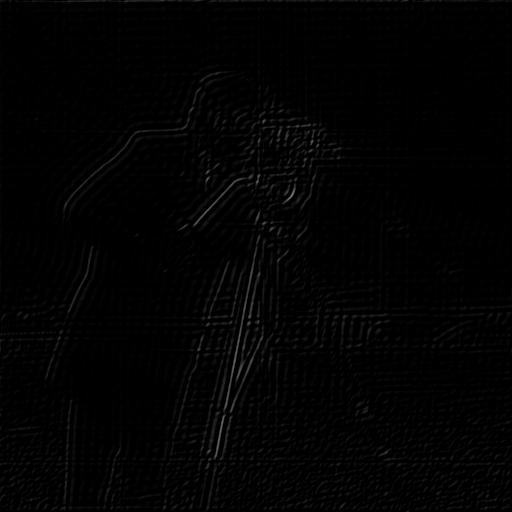
\includegraphics[width=0.32\textwidth]{img/edge_detect/camera_DL=015_DH=06_A=90_P=10}
  	}
  \subfloat[$D_L=0.15$, $D_H=0.6$, $\alpha = 90 \deg$, $P(1;1)$]{
    \label{fig_wyniki:edgeC1}
  		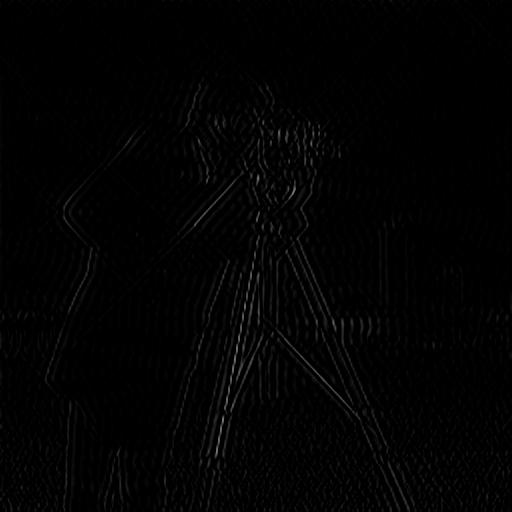
\includegraphics[width=0.32\textwidth]{img/edge_detect/camera_DL=015_DH=06_A=90_P=11}
  	}
  \caption{Filtr pasmowozaporowy.}
    \label{fig_wyniki:edge1}
\end{figure}



 \begin{figure}[H]
  \centering
  \subfloat[$D_L=0.15$, $D_H=0.6$, $\alpha = 30 \deg$, $P(1;1)$]{
    \label{fig_wyniki:edgeC2}
	  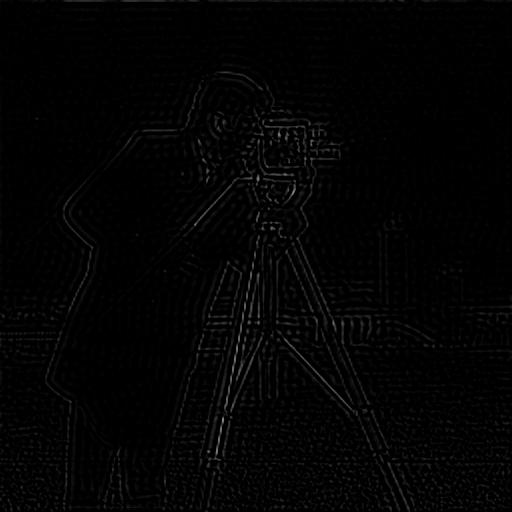
\includegraphics[width=0.33\textwidth]{img/edge_detect/camera_DL=015_DH=06_A=30_P=11}
  }
  \subfloat[$D_L=0.15$, $D_H=0.6$, $\alpha = 120 \deg$, $P(1;1)$]{
    \label{fig_wyniki:edgeC3}
  		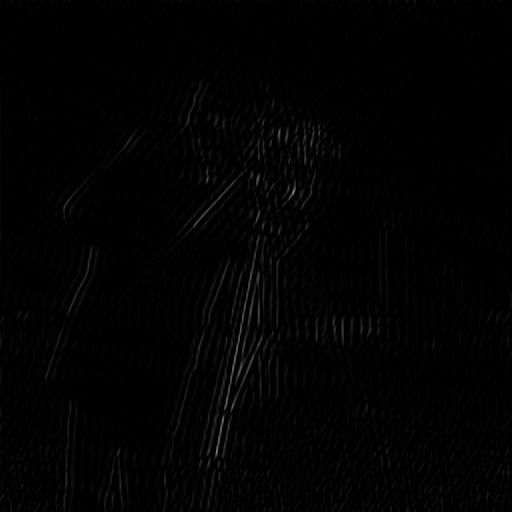
\includegraphics[width=0.33\textwidth]{img/edge_detect/camera_DL=015_DH=06_A=120_P=11}
  	}
  \caption{Filtr pasmowozaporowy, różne kąty dla $P(1;1)$.}
    \label{fig_wyniki:edge2}
\end{figure}



\subsubsection{Filtr modyfikujący widmo}



 \begin{figure}[H]
  \centering
  \subfloat[$l=0.25$, $k=0.25$]{
    \label{fig_wyniki:modyfikacjaA}
	  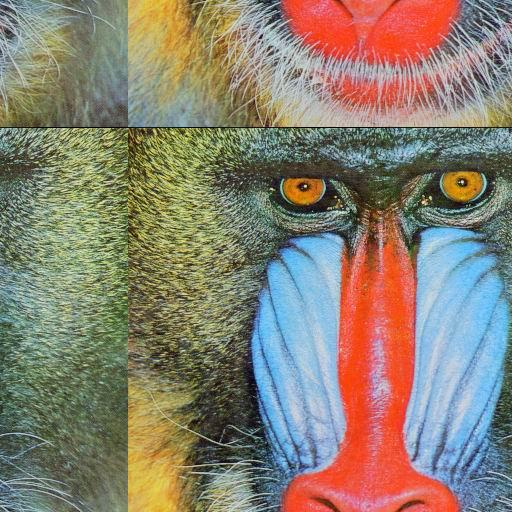
\includegraphics[width=0.33\textwidth]{img/modyfikacja/mandril_l025_k025}
  }
  \subfloat[$l=0.25$, $k=0.5$]{
    \label{fig_wyniki:modyfikacjaB}
  		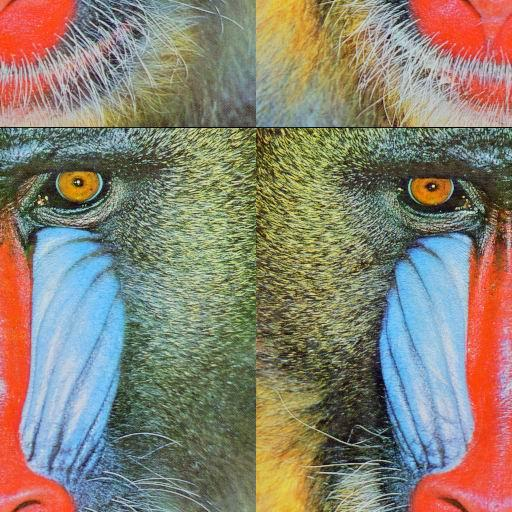
\includegraphics[width=0.33\textwidth]{img/modyfikacja/mandril_l025_k05}
  	}
  \caption{Filtr modyfikujący widmo.}
    \label{fig_wyniki:modyfikacja}
\end{figure}



\subsection{Segmentacja}
W opisach wyników obrazów segmentacji posłużyliśmy się oznaczeniami:
\begin{itemize}
\item $T$ - zastosowany współczynnik tolerancji dla zadanej metody
\item $M$ - ilość masek przedstawiona na obrazie
\item $M_{min}$ - minimalna ilość pikseli znajdująca się w masce
\end{itemize}

Testy dla obrazów w skali szarości zostały przeprowadzone dla obrazu \textit{bird}, natomiast dla obrazów kolorowych wybrano \textit{lena}. W sprawozdaniu zostały umieszczone obrazy przedstawiające wszystkie maski, każdą osobnym kolorem. Nasz program ma oczywiście możliwość eksportu tych masek jako osobnych czarno--białych grafik, lub podglądu ich na obrazie w trybie przezroczystości i bez niej oraz odwrotności danej maski.

 \begin{figure}[H]
  \centering
  \subfloat[Metoda Euklidesowa. $T$=21,$M$=11, $M_{min}$=2000px ]{
    \label{fig_wyniki:seg_bird1}
	  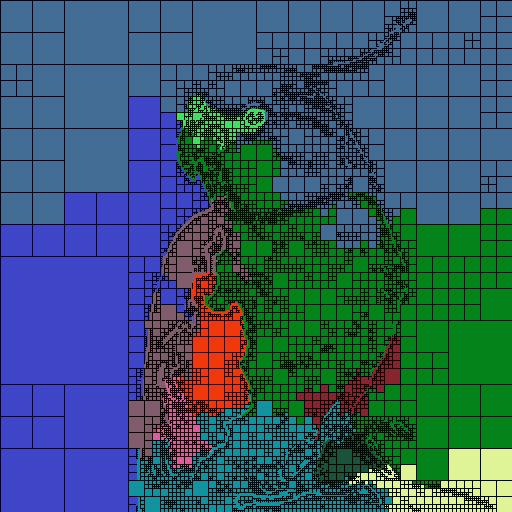
\includegraphics[width=0.37\textwidth]{img/seg/mask/bird/Simple21_2000_11}
  }
  \subfloat[Porównanie jasności. $T$=21,$M$=4, $M_{min}$=2000px ]{
    \label{fig_wyniki:seg_bird2}
  		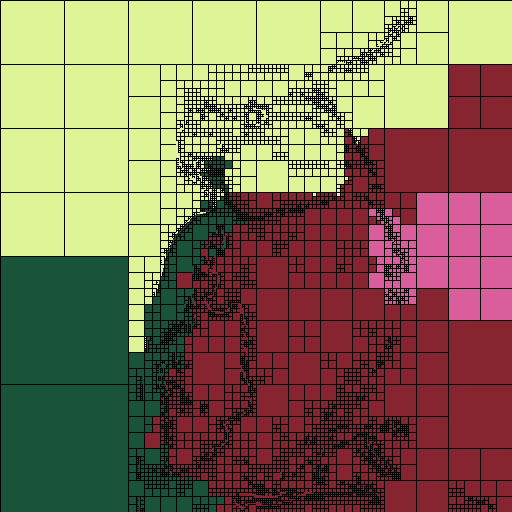
\includegraphics[width=0.37\textwidth]{img/seg/mask/bird/Luminace21_2000_4}
  	}
  	\\
  	  \subfloat[Odwrotność maski z przezroczystością.]{
    \label{fig_wyniki:seg_bird3}
	  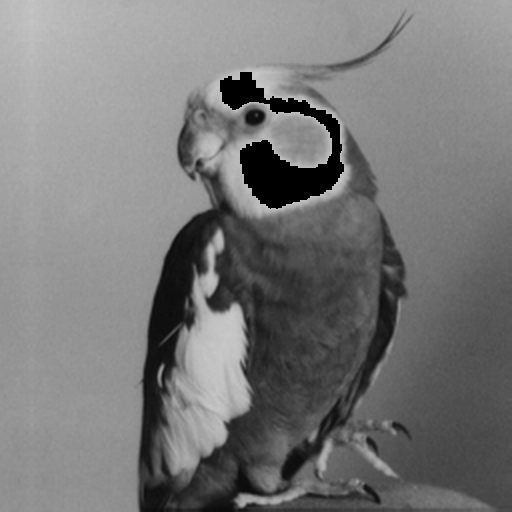
\includegraphics[width=0.37\textwidth]{img/seg/mask/bird/BirdMaskInverse_transparent}
  }
  \subfloat[Bało--czarna maska.]{
    \label{fig_wyniki:seg_bird4}
  		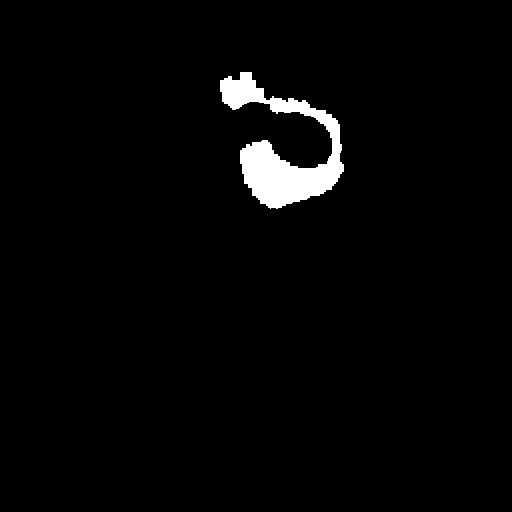
\includegraphics[width=0.37\textwidth]{img/seg/mask/bird/BirdMaskFill}
  	}
  \caption{Przykłady segmentacji obrazu \textit{bird}.}
  \label{fig_wyniki:seg_bird}
\end{figure}

\begin{figure}[H]
  \centering
  \subfloat[$T$=10, $M$=3127]{
    \label{fig_wyniki:seg_birds1}
	  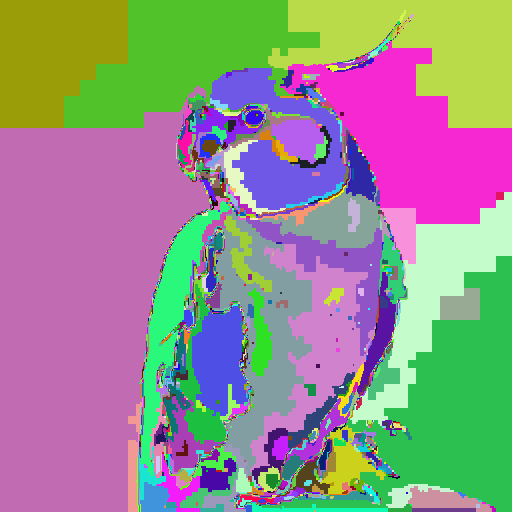
\includegraphics[width=0.37\textwidth]{img/seg/mask/bird/BirdSimpleT=10_all_3127}
  }
  \subfloat[$T$=10, $M$=33, $M_{min}$=1000px]{
    \label{fig_wyniki:seg_birds2}
  		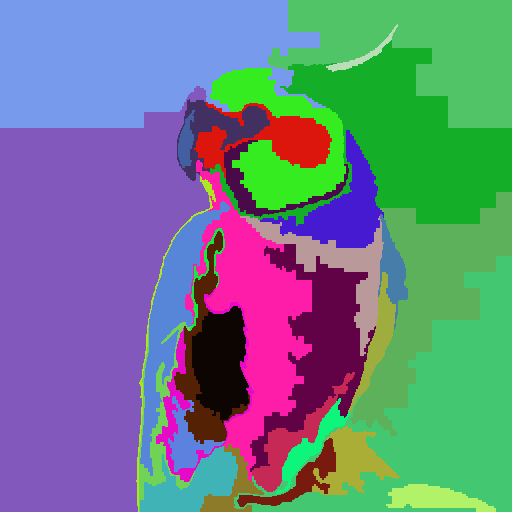
\includegraphics[width=0.37\textwidth]{img/seg/mask/bird/BirdSimpleT=10_33_1000}
  	}
  	\\
  	\subfloat[$T$=10, $M$=21, $M_{min}$=2000px]{
    \label{fig_wyniki:seg_birds3}
	  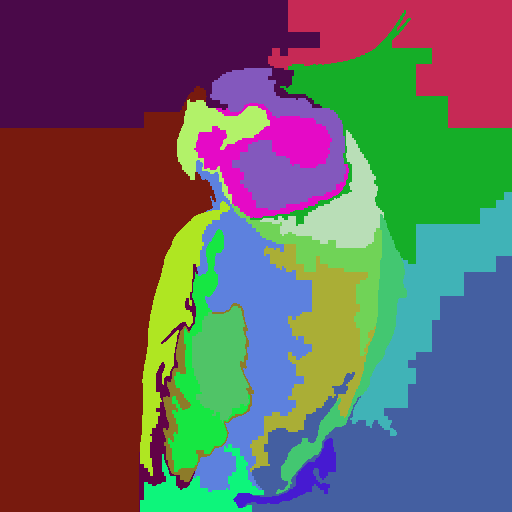
\includegraphics[width=0.37\textwidth]{img/seg/mask/bird/BirdSimpleT=10_21_2000}
  }
  \subfloat[$T$=5, $M$=29, $M_{min}$=4000px]{
    \label{fig_wyniki:seg_birds4}
  		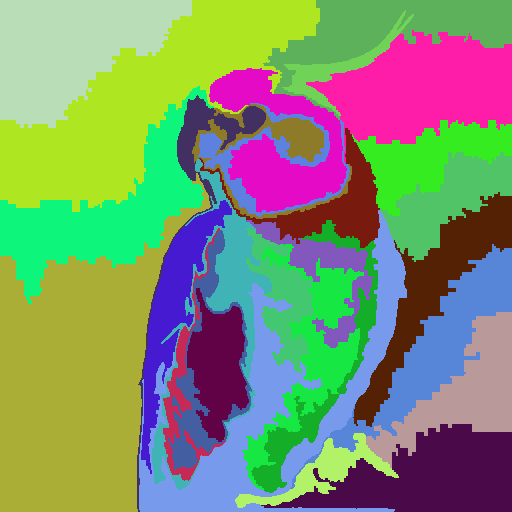
\includegraphics[width=0.37\textwidth]{img/seg/mask/bird/BirdSimpleT=5_29_4000}
  	}
  \caption{Segmentacja obrazu \textit{bird}. Metoda prosta dla każdego kanału.}
  \label{fig_wyniki:seg_birds}
\end{figure}

\begin{figure}[H]
  \centering
  \subfloat[$T$=10, $M$=16634]{
    \label{fig_wyniki:seg_lenas1}
	  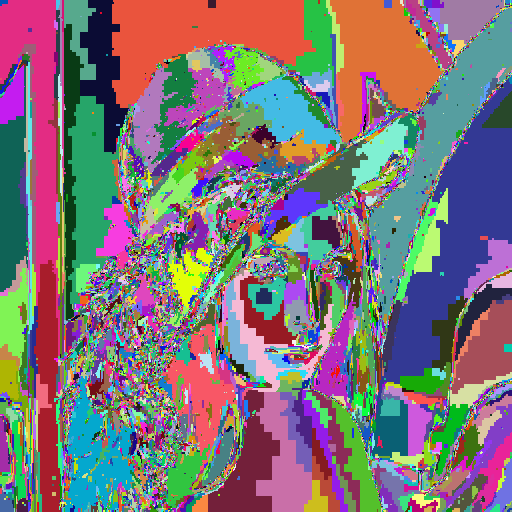
\includegraphics[width=0.37\textwidth]{img/seg/mask/lena/LenaSimpleT=10_16634}
  }
  \subfloat[$T$=10, $M$=118, $M_{min}$=1000px]{
    \label{fig_wyniki:seg_lenas2}
  		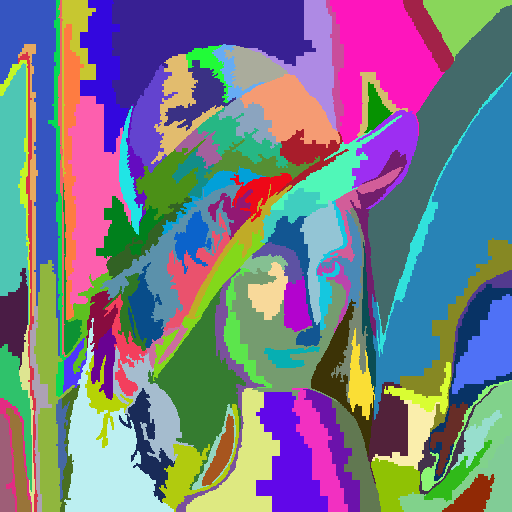
\includegraphics[width=0.37\textwidth]{img/seg/mask/lena/LenaSimpleT=10_118_1000}
  	}
  	\\
  	\subfloat[$T$=10, $M$=63, $M_{min}$=2000px]{
    \label{fig_wyniki:seg_lenas3}
	  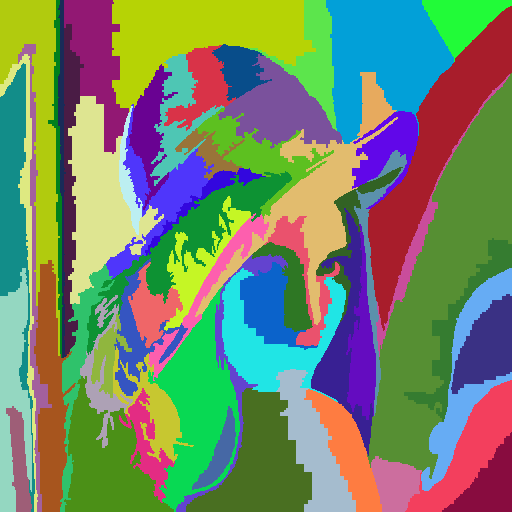
\includegraphics[width=0.37\textwidth]{img/seg/mask/lena/LenaSimpleT=10_63_2000}
  }
  \subfloat[$T$=5, $M$=45, $M_{min}$=4000px]{
    \label{fig_wyniki:seg_lenas4}
  		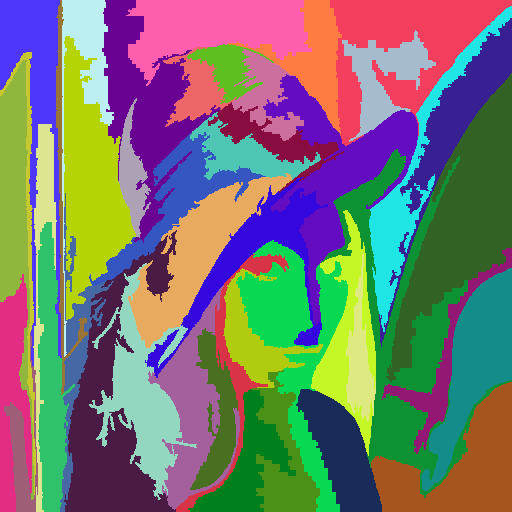
\includegraphics[width=0.37\textwidth]{img/seg/mask/lena/LenaSimpleT=5_45_4000}
  	}
  \caption{Segmentacja obrazu \textit{lena}. Metoda prosta dla każdego kanału.}
  \label{fig_wyniki:seg_lenas}
\end{figure}

\begin{figure}[H]
  \centering
  \subfloat[$T$=10,$M$=11981]{
    \label{fig_wyniki:seg_lenal1}
	  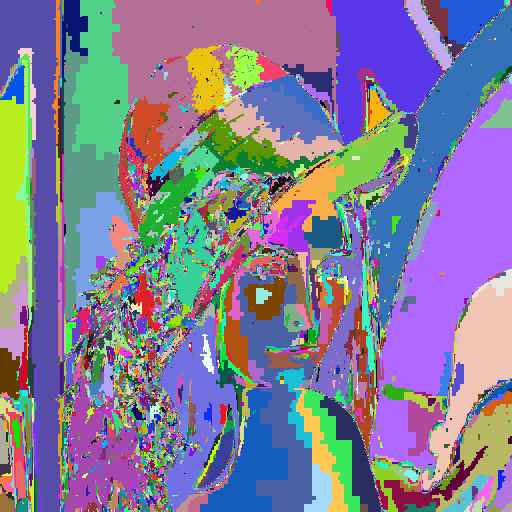
\includegraphics[width=0.37\textwidth]{img/seg/mask/lena/LenaLuminanceT=10_11981}
  }
  \subfloat[$T$=10, $M$=93, $M_{min}$=1000px]{
    \label{fig_wyniki:seg_lenal2}
  		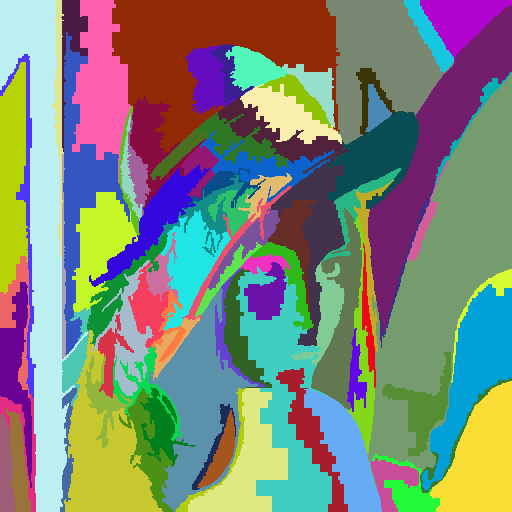
\includegraphics[width=0.37\textwidth]{img/seg/mask/lena/LenaLuminanceT=10_93_1000}
  	}
  	\\
  	\subfloat[$T$=10, $M$=52,$M_{min}$=2000px]{
    \label{fig_wyniki:seg_lenal3}
	  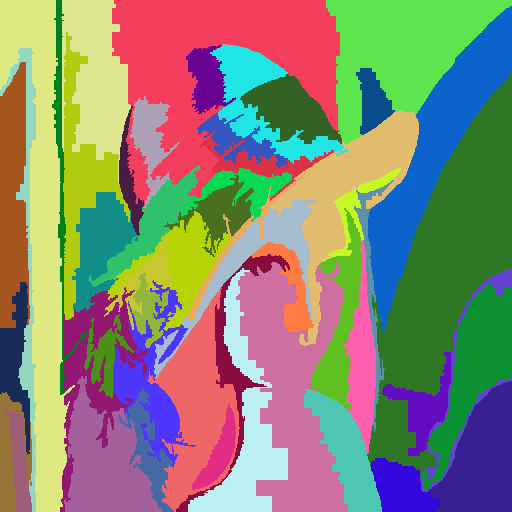
\includegraphics[width=0.37\textwidth]{img/seg/mask/lena/LenaLuminanceT=10_52_2000}
  }
  \subfloat[$T$=5, $M$=41, $M_{min}$=4000px]{
    \label{fig_wyniki:seg_lenal4}
  		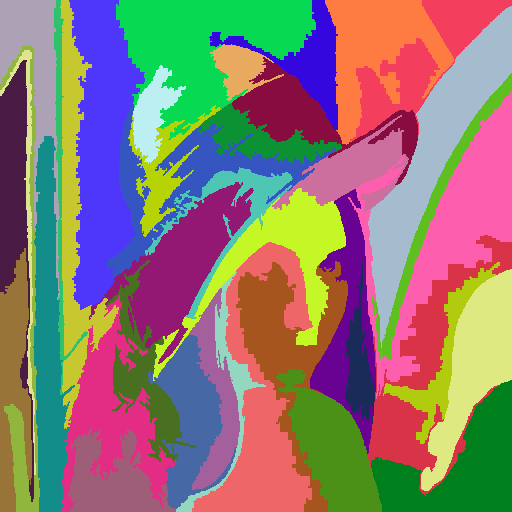
\includegraphics[width=0.37\textwidth]{img/seg/mask/lena/LenaLuminanceT=5_41_4000}
  	}
  \caption{Segmentacja obrazu \textit{lena}. Metoda porównania jasności.}
  \label{fig_wyniki:seg_lenal}
\end{figure}

\begin{figure}[H]
  \centering
  \subfloat[$T$=10, $M$=29032]{
    \label{fig_wyniki:seg_lenae1}
	  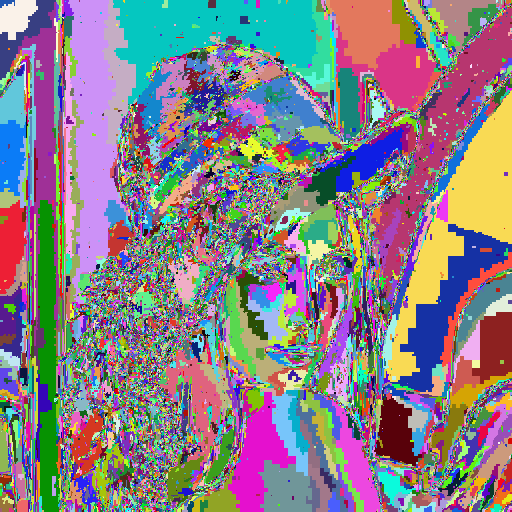
\includegraphics[width=0.37\textwidth]{img/seg/mask/lena/LenaEuclideanT=10_29032}
  }
  \subfloat[$T$=10, $M$=147, $M_{min}$=1000px]{
    \label{fig_wyniki:seg_lenae2}
  		\includegraphics[width=0.37\textwidth]{img/seg/mask/lena/LenaEuclideanT=10_147_1000}
  	}
  	\\
  	\subfloat[$T$=10, $M$=83, $M_{min}$=2000px]{
    \label{fig_wyniki:seg_lenae3}
	  \includegraphics[width=0.37\textwidth]{img/seg/mask/lena/LenaEuclideanT=10_83_2000}
  }
  \subfloat[$T$=5, $M$=58, $M_{min}$=4000px]{
    \label{fig_wyniki:seg_lenae4}
  		\includegraphics[width=0.37\textwidth]{img/seg/mask/lena/LenaEuclideanT=5_58_4000}
  	}
  \caption{Segmentacja obrazu \textit{lena}. Metoda Euklidesowa.}
  \label{fig_wyniki:seg_lenae}
\end{figure}



\section{Dyskusja}

\subsection{Filtracja w dziedzinie częstotliwości}

\subsubsection{Filtr dolnoprzepustowy}

Dzięki temu filtrowi uzyskujemy efekt rozmycia, jak widać na rysunku \ref{fig_wyniki:lp}. Jednak im bardziej rozmyjemy obraz(im niższa wartość parametru $D_0$) tym bardziej widoczne stają się artefakty widoczne na rys \ref{fig_wyniki:lpA}. Jednak stosując filtr Butterwortha, można te niepożądane efekty zniwelować(rys. \ref{fig_wyniki:lpB});

\subsubsection{Filtr górnoprzepustowy}

Filtr ten jest negacją filtru poprzedniego, więc jak się można spodziewać efekt będzie odwrotny jak w tamtym przypadku czyli wyostrzenie. Parametr $D_0$ w wyższych wartościach powoduje pozostawienie na obrazie jedynie najwyraźniejszych krawędzi obrazu (rys. \ref{fig_wyniki:hpA}), a przy coraz mniejszych wartościach odwrotnie, czyli uwydatnianie krawędzi, obiektów wyróżniających się, kontrastujących z ich tłem (rys. \ref{fig_wyniki:hpB}) .

\subsubsection{Filtr pasmowoprzepustowy}

Filtr ten daje podobny efekt jak w przypadku filtru górnoprzepustowego przy obraniu wysokich wartości parametrów  $D_L$ $D_H$.

Jednak w odróżnieniu od niego pozwala na wybranie interesującego nas pasma częstotliwości branego pod uwagę. Można uzyskać nim lepszy wynik przy wyostrzaniu obrazów  rys. \ref{fig_wyniki:bp_boat}  rys. \ref{fig_wyniki:bp_lena}. Porównując wynik uzyskany za pomocą filtru idealnego i filtru Butterwortha widać, że obcinając ,,zero-jedynkowo'' przedział częstotliwości, w znacznym stopniu zmieniamy obraz wynikowy w stosunku do wejściowego. Przejścia pomiędzy obszarami jasności a obszarami ciemnymi stają się bardziej skokowe, natomiast stosując filtr Butterwortha zachowują więcej odcieni szarości - zachowane jest ciągłe przejście.


\subsubsection{Filtr pasmowozaporowy}

Podobnie jak w przypadku filtru dolnoprzepustowego i górnoprzepustowego, filtr ten jest negacją filtru pasmowoprzepustowego. Ciekawy efekt jaki udało się uzyskać stosując ten filtr jest wygładzenie, rozmycie obrazu z jednoczesnym zachowaniem wyraźnych krawędzi (rys. \ref{fig_wyniki:bs}). Podobnie jak w przypadku filtru dolnoprzepustowego, zastosowanie filtracji Butterwotha pozwala nam uniknąć artefaktów powstałych w przypadku filtracji idealnej.

\subsubsection{Filtr z detekcją krawędzi}

Analogicznie jak w przypadku wykrywania krawędzi zaprezentowanego w zadaniu pierwszym. Filtr ten pozwala na wykrycie linii oraz krzywych, jednak w odróżnieniu do tamtego rozwiązania filtr ten pozwala na zdefiniowane zakresu krzywizny identyfikowanych krzywych poprzez parametry $\alpha$ oraz $P$ (punkt ramienia kąta o wierzchołku w (0,0)). Jak widać na rysunkach \ref{fig_wyniki:edge1} gdzie dla ustalonego kąta zmieniamy ramie kąta, zmieniamy orientacje wykrywanych krzywych. Oraz zmieniając kąt (rys. \ref{fig_wyniki:edge2}) zmieniamy zakres krzywizny.

\subsubsection{Filtr modyfikujący widmo}

W odróżnieniu do filtrów opisanych powyżej filtr ten nie polega na odrzuceniu pewnego pasma częstotliwości, lecz przemnaża cały obraz przez filtr $H$ \ref{eq:modyfikacja}. W wyniku otrzymujemy przesunięty cyklicznie obraz względem obu osi, przesunięcie to jest zdefiniowane za pomocą parametrów \emph{l}, \emph{k}.



\subsection{Segmentacja}
Zaimplementowane metody porównywania pikseli oraz obszarów nie mają znaczenia w przypadku obrazów w skali szarości. Każda z nich zwraca taki sam wynik przy takim samym współczynniku tolerancji. Jedyna zauważalna różnica to czas potrzebny do wygenerowania poszczególnych masek każdą z tech metod. Prosta metoda porównania koloru dla jednego kanału jest najszybsza natomiast Metoda Euklidesowa najwolniejsza. W sprawozdaniu zostały zamieszczone jedynie efekty pracy dla najszybszego algorytmu. 

Dla obrazu \ref{fig_wyniki:seg_birds1} dla początkowej segmentacji z $T=10$ bez dodatkowych ograniczeń ilość powstałych masek jest bardzo dużo i wynosi 3127. Dzieję się tak dlatego, że nawet mimo zastosowania pewnej tolerancji poszczególne komórki mogą być nadal bardzo mało a ich porównanie z otaczającymi może nie pozwalać na ich połączenie. Widać znacząc poprawę dla obrazów gdzie zastosowaliśmy współczynniki dodatkowo jeszcze zmuszające łączenie małych masek. Obrazy te są bardziej jednolite a ilość uzyskanych masek jest mniejsza [\ref{fig_wyniki:seg_birds2},\ref{fig_wyniki:seg_birds3}]. Przy zmniejszeniu progu tolerancji o połowę i przy jednoczesnym podniesieniu wartości minimalnej ilość pikseli w masce ich ilość wzrosła w porównaniu do wcześniejszych prób \ref{fig_wyniki:seg_birds4}.

W przypadku obrazów kolorowych segmentacja bez ograniczenia w postaci minimalnej ilości w pikseli w masce zwróciła zawsze bardzo dużo osobnych obszarów. Ma to związek z samym obrazem użytym do przeprowadzenia badań, na którym to występuje dużo zróżnicowanych obiektów. Szczególnie trudne w segmentacji okazują się być włosy, gdzie skupiło się wiele małych masek \ref{fig_wyniki:seg_lenas1}. Ale tak samo jak w przypadku obrazów w skali szarości dodanie parametru określającego minimalną wielkość maski pomogło zredukować ich liczbę oraz połączyć je w większe grupy [\ref{fig_wyniki:seg_lenas2},\ref{fig_wyniki:seg_lenas3},\ref{fig_wyniki:seg_lenas4}].

\section{Wnioski}

\subsection{Filtracja w dziedzinie częstotliwości}

Transformacja obrazu do dziedziny częstotliwości pozwala na wykonanie wielu filtracji obrazu w mniej zachłanny sposób. Najlepszym przykładem tutaj będzie porównanie filtru uśredniającego z filtrem dolnoprzepustowym do zadania rozmycia obrazu. Gdy chcemy uzyskać większe rozmycie w przypadku filtru uśredniającego należałoby zwiększyć maskę co z kolei zwiększałoby ilość potrzebnych obliczeń. Natomiast gdy operujemy filtrem dolnoprzepustowym, nie zwiększy to w żaden sposób ilości obliczeń, dzięki temu uzyskujemy dobrze skalującą się metodę. W zależności od zastosowania, dobrym pomysłem może być zastosowanie filtrów o charakterystykach innych od idealnej, na przykładzie zastosowanego w zadaniu filtru Butterwortha można zauważyć, że przy zastosowaniu filtru idealnego mogą wystąpić niepożądane efekty tj na rys. \ref{fig_wyniki:lpA} , \ref{fig_wyniki:bp_boatA} oraz \ref{fig_wyniki:bsA}. 


\subsection{Segmentacja}

Segmentacja obrazu przy pomocy drzewa czwórkowego pozwala w efektywny sposób na jego podział na rejony o podobnej charakterystyce. Dzięki wykorzystaniu przez nas szybkiej metody znajdowania sąsiadów czas pracy algorytmu jest krótszy niż w przypadku innych standardowych rozwiązań. Dodanie jednak dodatkowego czynnika jakim jest minimalna wielkość wygenerowanej maski wydłuża obliczenia i spowalnia cały proces. Jednak bez tego kroku uzyskane rezultaty można oceniać jako mało zadowalające. Następuje wtedy zbyt drobna segmentacja obrazu co skutkuje powstaniem dużej ilości masek, które nie reprezentują przeważnie całego obiektu, lub jego charakterystycznej części. 

Dzięki możliwości ,,zmuszenia'' algorytmu do podziału do zadanej głębokości można osiągnąć efekt podobny do metody rozrostu, zaproponowanej jako pierwszy wariant tego zadania. Niestety ze względu na konieczność wygenerowania wszystkich komórek na starcie algorytmu powoduje, że czas przetwarzania się wydłuża. Metoda ta przez to nie najlepiej spisuję się w tym zastosowaniu.

Dzięki temu że w naszej metodzie segmentacji obliczamy średni kolor obrazu dla każdej utworzonej maski może ona posłużyć po dobraniu odpowiednich parametrów jaki swoisty rodzaj kompresji. Obraz byłby wtedy przechowywany jako spis pól, gdzie każdemu z nich przypisany byłby osobny kolor. Jest to oczywiście kompresja stratna, która ma może mieć bardzo duży wpływ na jakoś obrazu a przy niewłaściwych parametrach obraz wyjściowy może zajmować więcej miejsca niż obraz początkowy.

\begin{thebibliography}{8}

\bibitem{1} Fast Fourier Transform (FFT) \url{http://www.cmlab.csie.ntu.edu.tw/cml/dsp/training/coding/transform/fft.html}
\bibitem{2} The Radix 2 Decimation In Frequency (DIF) Algorithm.  \url{http://www.engineeringproductivitytools.com/stuff/T0001/PT03.HTM}
\bibitem{3} Constant Time Neighbor Finding in Quadtrees: An Experimental Result, Kunio Aizawa, Koyo Motomura, Shintaro Kimura, Ryosuke Kadowaki, and Jia Fan
\end{thebibliography}

\end{document}
